\documentclass[varwidth=true, border=2pt]{standalone}

\usepackage{pgfplots}
\usepackage{tikz}
\usetikzlibrary{shapes.geometric}

\usetikzlibrary{calc,patterns,angles,quotes}

\begin{document}

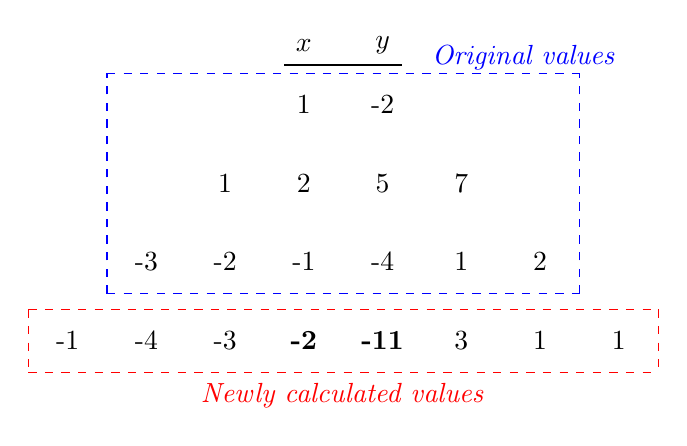
\begin{tikzpicture}[square/.style={regular polygon,regular polygon sides=4}]


	\node (A) at (1.5,3.25) {$x$};
	\node  (B) at (1.5,2.5){1}; 
	\node (C) at (1.5,1.5) {2};
	\node (D) at (1.5,0.5) {-1};
	\node (E) at (1.5, -0.5) {\textbf{-2}};
	\node (F)at (0.5,1.5) {1};
	\node (G) at (0.5,0.5) {-2};
	\node (H) at (0.5, -0.5) {-3};
	\node (I) at (-0.5,0.5) {-3};
	\node (J) at (-0.5, -0.5) {-4};
	\node (K) at (-1.5, -0.5) {-1};
	\node (a) at (2.5,3.25) {$y$};
	\node (b) at (2.5,2.5) {-2};
	\node  (c) at (2.5,1.5) {5};
	\node  (d) at (2.5,0.5) {-4};
	\node (e)  at (2.5, -0.5) {\textbf{-11}};
	\node (f)  at (3.5,1.5) {7};
	\node (g) at (3.5,0.5) {1};
	\node (h) at (3.5,-0.5) {3};
	\node (i) at (4.5, 0.5) {2};
	\node (j) at (4.5, -0.5) {1};
	\node (k) at (5.5, -0.5) {1};
	\node (l)[red] at (2, -1.2) {\textit{Newly calculated values}};
	\node (m) [blue] at (4.3, 3.1) {\textit{Original values}};

	\draw [thick, black] (1.25,3) to (2.75,3);
	\draw [red, dashed] (-2,-0.1) to (6,-0.1);
	\draw [red, dashed] (-2,-0.9) to (6,-0.9);
	\draw [red, dashed] (-2,-0.1) to (-2,-0.9);
	\draw [red, dashed] (6,-0.1) to (6,-0.9);
	\draw [blue, dashed] (-1, 0.1) to (5, 0.1);
	\draw [blue, dashed] (-1, 2.9) to (5, 2.9);
	\draw [blue, dashed] (-1, 0.1) to (-1, 2.9);
	\draw [blue, dashed] (5, 0.1) to (5, 2.9);
\normalsize

\end{tikzpicture}
\end{document}